\section{升力阻力性能}

\subsection{升力阻力特性概述}

在给定巡航高度$h$的和飞行马赫数$Ma$的情况下,
全机所受的飞行升力与阻力可以用飞行器的动压、机翼参考面积和一个比例系数进行表示:
\begin{equation}
    \begin{cases}
        \begin{aligned}
            L&=\frac{1}{2}C_L \rho Ma^2 c^2 S\\
            D&=\frac{1}{2}C_D \rho Ma^2 c^2 S
        \end{aligned}
    \end{cases}
\end{equation}

其中$\rho = \rho_{\infty}$,$c = c_{\infty}$为巡航高度上的密度和声速,
$S$为参考面积,
$C_L$和$C_D$是升力系数与阻力系数。

\subsubsection{升力特性概述}

在给定的飞行状态下,
全机的升力系数小迎角范围内(取$-4\sim 8 ^{\circ}$),
是迎角的一次函数:
\begin{equation}
    \label{升力线斜率关系}
    C_L = C_{l\alpha} (\alpha - \alpha_0)
\end{equation}

其中$C_{l\alpha}$是全机升力系数斜率,是表征升力特性的一个重要气动参数:
\begin{equation}
    C_{l\alpha}= C_{l\alpha}(Ma) = \frac{\partial C_L}{\partial \alpha} 
\end{equation}

在该飞机的外形参数确定时,
$C_{l\alpha}$仅是飞行马赫数$Ma$的参数。
其中$\alpha_0$为零升迎角,表征没有升力时的迎角。

在给定的原始数据中,可以绘制出离散点上不同马赫数$Ma$下的升力系数$C_L$如\ref{升力系数原始数据}。

\begin{figure}[H]
    \centering
    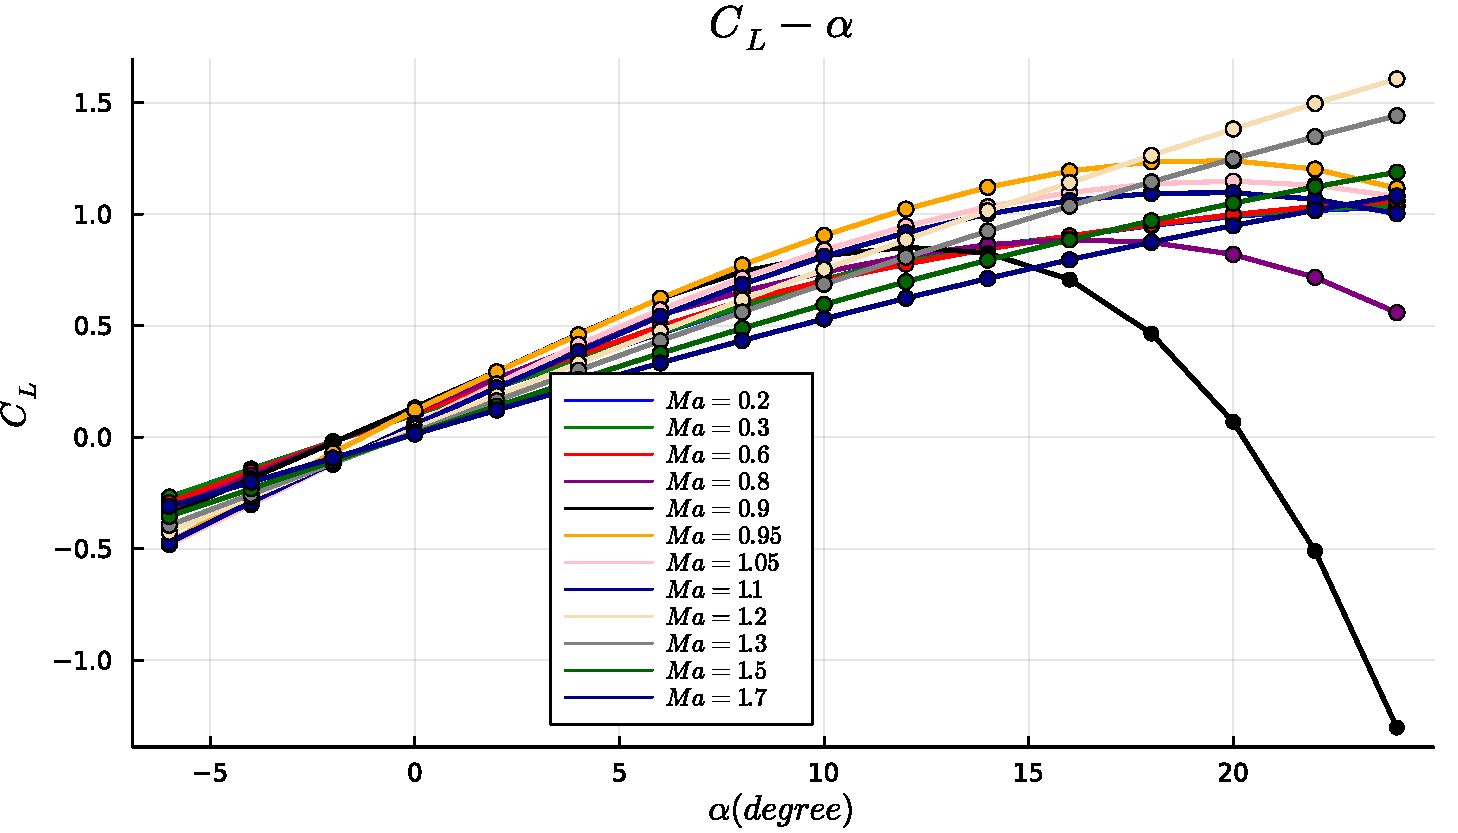
\includegraphics[width=0.9\textwidth]{image/ch3/CL_alpha_origin.pdf}
    \caption{升力系数$C_L-\alpha$原始数据}
    \label{升力系数原始数据}
\end{figure}

可以发现在角度较小的范围内,
基本呈线性关系。

\subsubsection{阻力特性概述}

在给定的飞行状态下,
升力系数$C_L$和阻力系数$C_D$呈二次关系,
在飞行计算中将$C_D$分成两部分:
为零升阻力部分$C_{D0}$和升至阻力部分$A$:
\begin{equation}
    \label{极曲线关系}
    C_D = C_{D0} + AC_{L}^2
\end{equation}

其中$C_{D0}$和$A$的参数受飞行马赫数$Ma$和雷诺数$Re$的影响。
通常来讲只认为零升阻力系数$C_{D0}$和$A$为马赫数$Ma$的函数。
如图\ref{升力阻力系数原始数据}中所示为原始数据。

\begin{figure}[H]
    \centering
    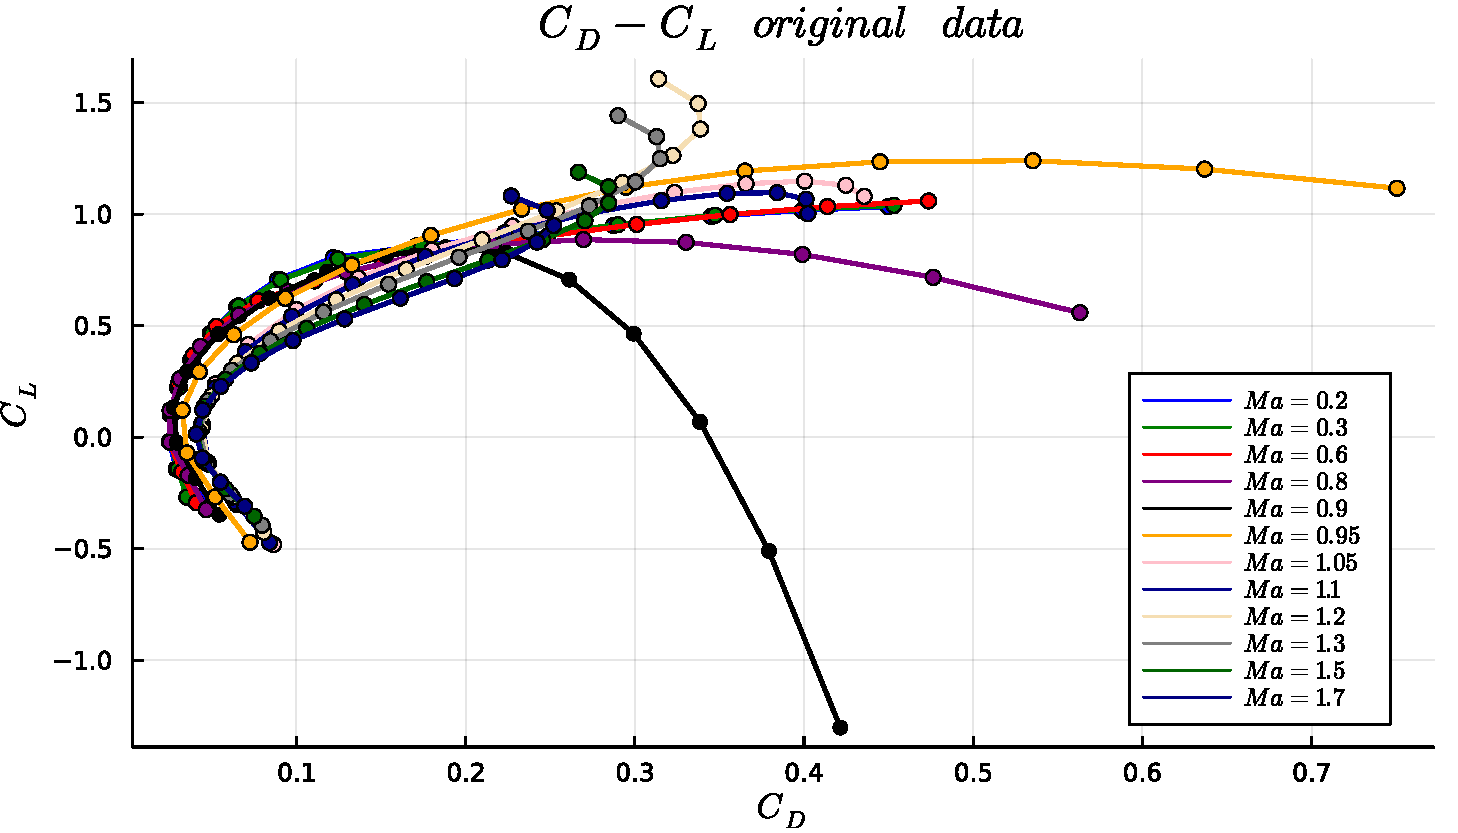
\includegraphics[width=0.9\textwidth]{image/ch3/CLCD_origin.pdf}
    \caption{升力阻力系数$C_L-C_D$原始数据}
    \label{升力阻力系数原始数据}
\end{figure}

可以发现,当$C_L$一定范围内(也即小迎角范围内),
$C_L$和$C_D$基本呈抛物线型,
也就是升力阻力特性的极曲线(drag polar)关系。




\subsection{不同马赫数下的全机升力系数斜率$C_{l\alpha}$}

如方程\ref{升力线斜率关系}中,
参数$C_{l\alpha}$在小迎角范围内可以视作一次函数关系方程的斜率。

利用最小二乘法如式\ref{最小二乘法}中的方法,
可以拟合不同马赫数$Ma$下的$C_{l\alpha}$的值。
在图\ref{升力系数原始数据}中选定某一个马赫数,
然后根据离散点上的值进行最小二乘拟合得到下述不同离散马赫数$C_{l\alpha}$值。

因为离散点上的值较为分散,
所以可以利用式\ref{样条插值}中的样条插值方法,
将离散数据点拟合成光滑而连续的分段曲线。
如图\ref{不同马赫数下的升力线斜率系数关系}中,
蓝色点为最小二乘法得到不同马赫数下的的升力线斜率系数离散值,
红色为样条插值函数。

容易发现升力线斜率系数在$Ma\approx 1.0$时达到最大值。
需要注意的是这里的$C_{l\alpha}$为角度取弧度制$rad$情况下对应的值。

\begin{figure}[H]
    \centering
    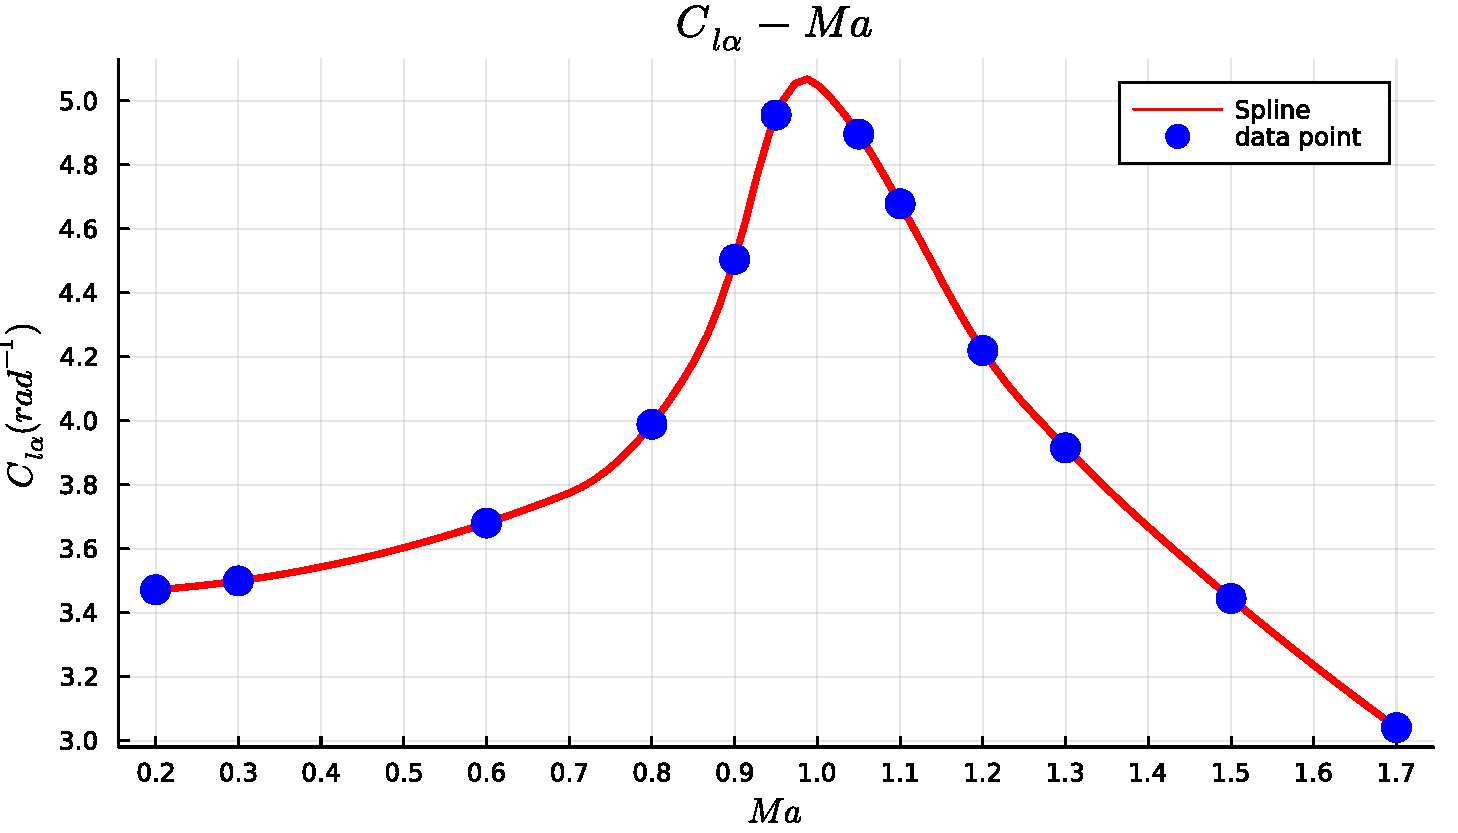
\includegraphics[width=0.6\textwidth]{image/ch3/Clalpha_Ma.pdf}
    \caption{不同马赫数下的升力线斜率系数$C_{l\alpha}-Ma$关系}
    \label{不同马赫数下的升力线斜率系数关系}
\end{figure}





\subsection{不同马赫数下的零升阻力系数$C_{D0}$}

在方程\ref{极曲线关系}中,
升力系数和阻力系数近似为一个$y = ax^2+b$的二次关系。
同样可以利用方程\ref{最小二乘法}最小二乘法中计算参数$C_{D0}$和$A$的值。

\begin{figure}[H]
    \centering
    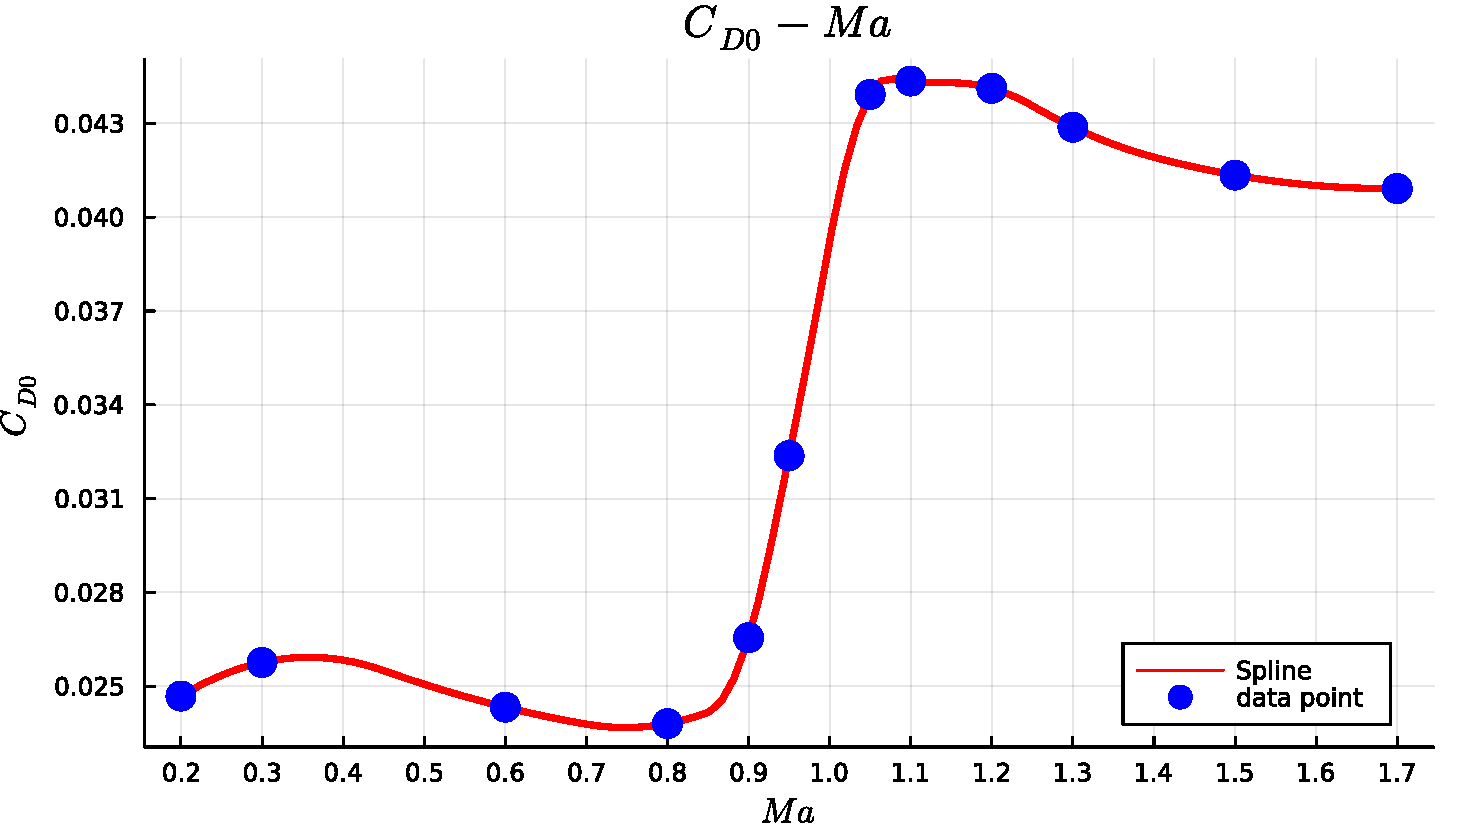
\includegraphics[width=0.6\textwidth]{image/ch3/CD0_Ma.pdf}
    \caption{不同马赫数下的零升阻力因子$C_{D0}-Ma$关系}
    \label{不同马赫数下的零升阻力因子关系}
\end{figure}

如图\ref{不同马赫数下的零升阻力因子关系}中为不同马赫数下的零升阻力因子$C_{D0}$。
蓝色的为离散点,
红色的为样条插值曲线。
容易发现在$Ma=1.0$附近,
$C_{D0}$的值有急剧的上升,
这就是音障现象,
在飞机飞行速度至音速时,
零升阻力部分会有急剧的增加。


\subsection{不同马赫数下的升致阻力因子$A$}

类似的,
在拟合得到$C_{D0}$时,
可以同时得到升致阻力因子系数$A$。
如下图所示

\begin{figure}[H]
    \centering
    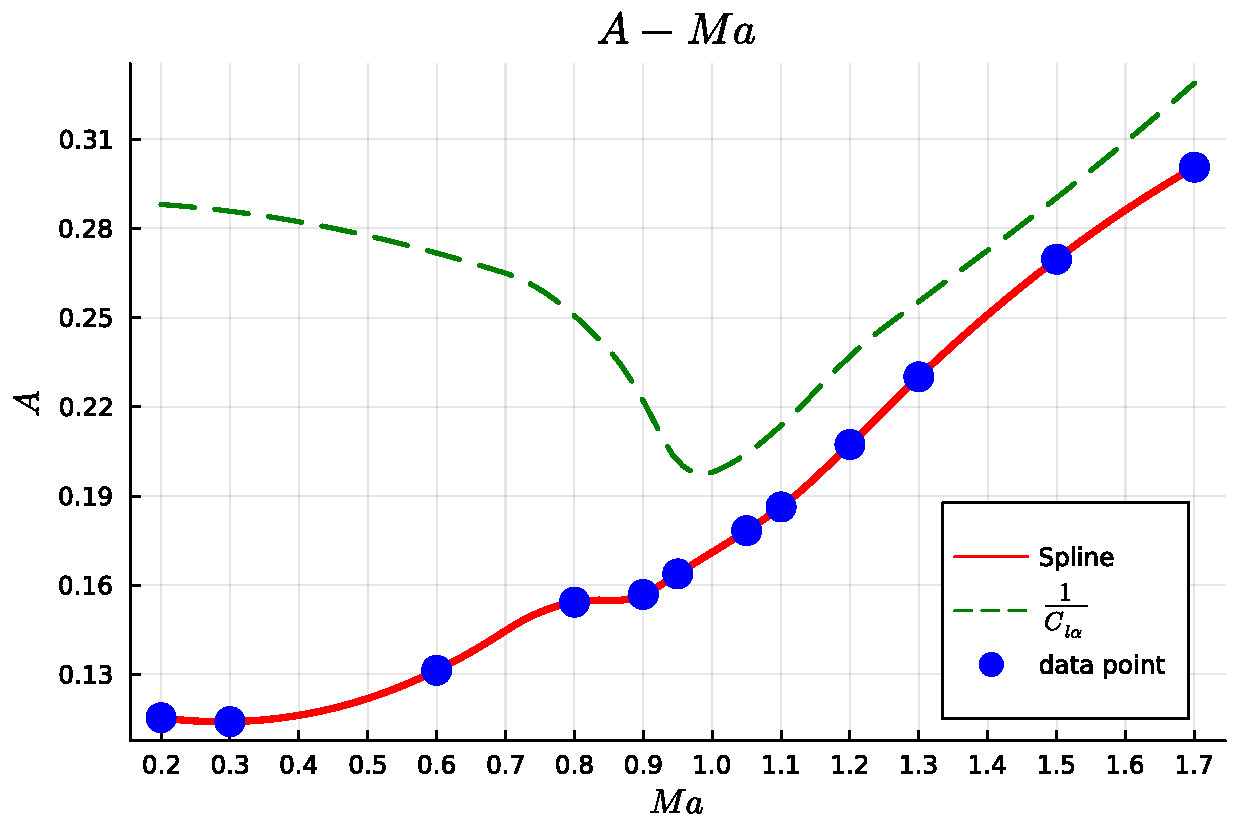
\includegraphics[width=0.6\textwidth]{image/ch3/A_Ma.pdf}
    \caption{不同马赫数下的升至阻力因子系数$A-Ma$关系}
    \label{不同马赫数下的升至阻力因子系数关系}
\end{figure}

$A$随着马赫数$Ma$的增加较为平稳地缓慢增加,
在马赫数$Ma$在$0.8\sim 1.0$时,
反而有一个稍微平稳的“台阶”。
另外值得注意的是,
在马赫数较大时,
$A$的发展趋势基本与$1/C_{l\alpha}$的趋势一致,
如图中绿色虚线部分。




\subsection{极曲线}

在前述不同马赫数$Ma$下的$C_{D0}$与$A$计算得到后,
可以将理论上的极曲线进行绘制、比较。
如式\ref{极曲线关系}中所示,
绘制不同飞行马赫数$Ma$下的升力系数$C_L$和阻力系数$C_D$关系为极曲线(polar curve)如图\ref{不同飞行马赫数Ma下的升力系数阻力系数极曲线}。
实线(拟合极曲线)与离散点(原始数据)吻合得较好。

\begin{figure}[H]
    \centering
    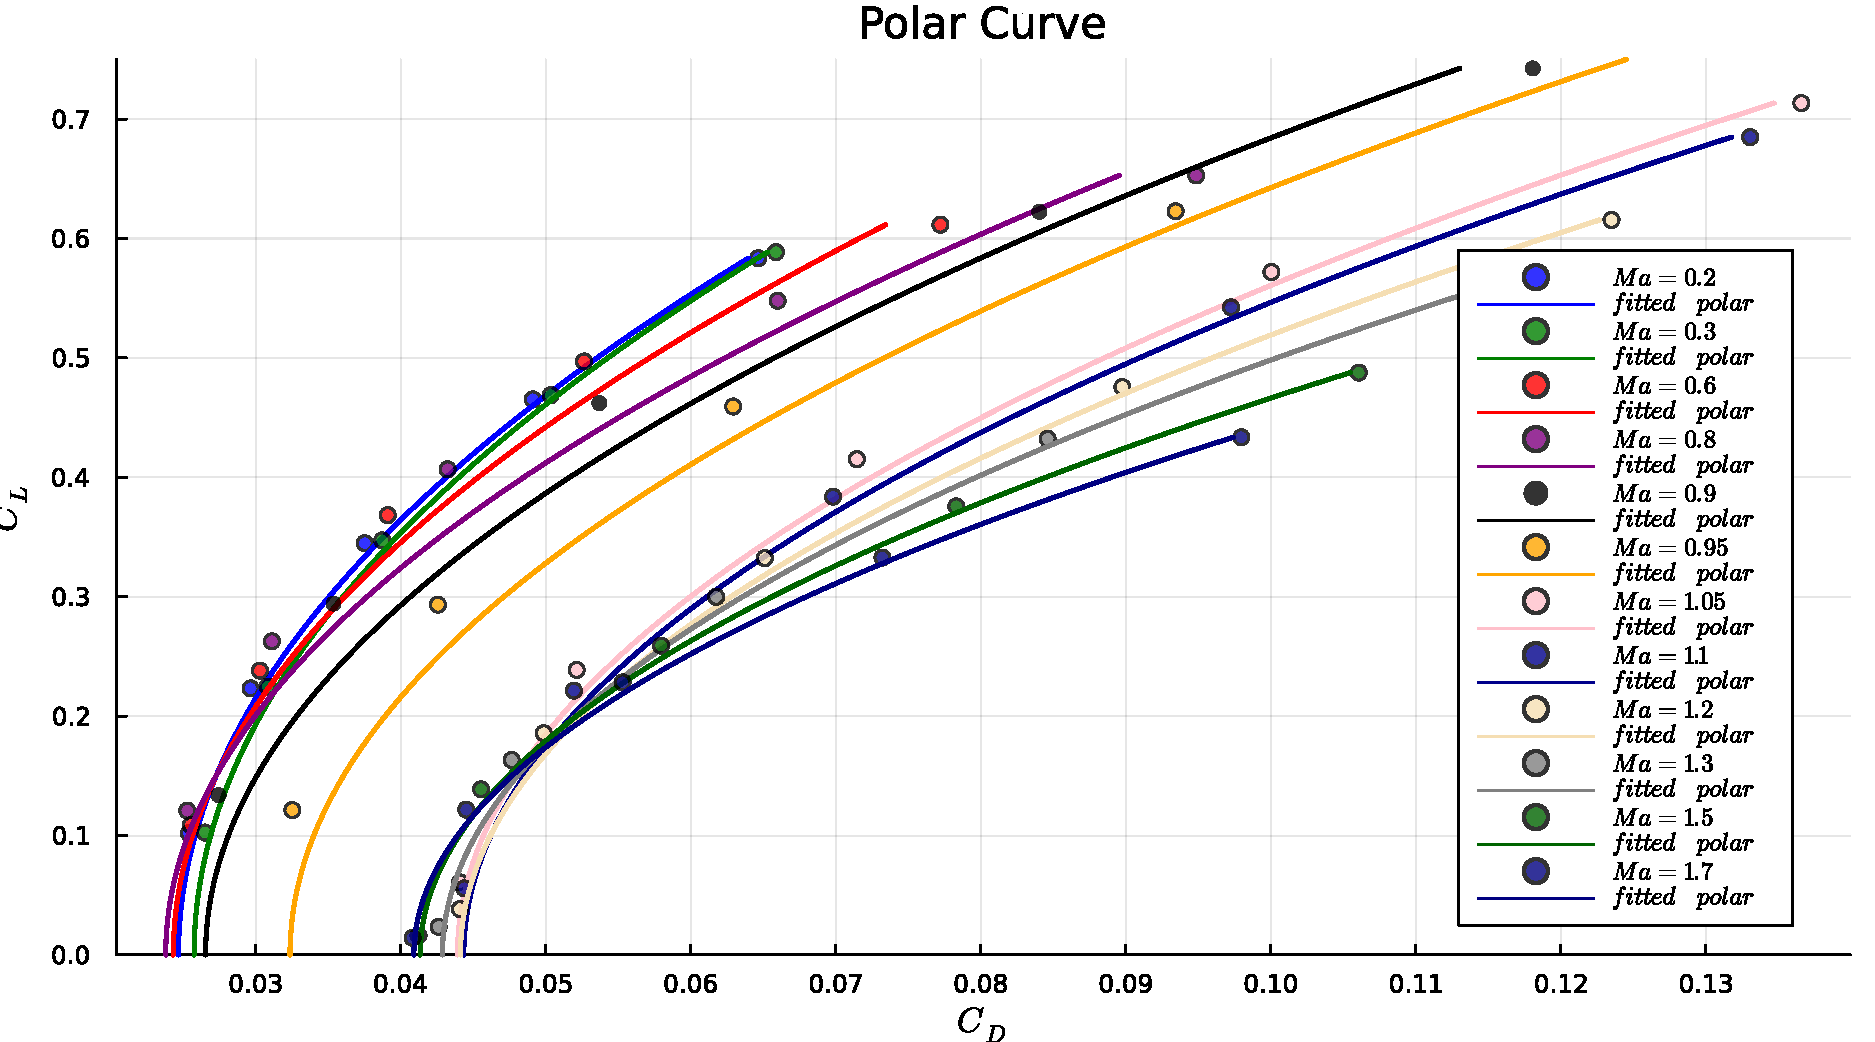
\includegraphics[width=0.9\textwidth]{image/ch3/drag_polar.pdf}
    \caption{不同飞行马赫数$Ma$下的升力系数阻力系数极曲线}
    \label{不同飞行马赫数Ma下的升力系数阻力系数极曲线}
\end{figure}